\documentclass[12pt]{article}
\usepackage{fullpage, graphicx, float}
\usepackage[page]{appendix}
\usepackage{extramarks}
\usepackage{algorithm}
\usepackage{algorithmic}
\usepackage{color}

%%%%%%%%%%%%%%%%%%%%%%%%%%%%%%%%%%%%%%%%%%%%%%%%%%%%%%%%%%%%%
% Homework Specific Information
\newcommand{\hmwkTitle}{Retriever Project}
\newcommand{\hmwkDueDate}{Sunday,\ May\ 10,\ 2009}
\newcommand{\hmwkClass}{4005-759-03\ Mobile Robots Programming}
\newcommand{\hmwkAuthorName}{Jeton\ Bacaj\ and Jeffrey\ Robble}
\newcommand{\hmwkClassInstructor}{4005-759-03 - Dr. Z. Butler}

% Make title
% textmd - medium text
\title{
  \vspace{2in}
  \textmd{\textbf{\hmwkTitle}} \\
  \vspace{0.1in}
  \large{\textmd{\hmwkClassInstructor}} \\
  \vspace{0.1in}
  \normalsize\small{Due\ on\ \hmwkDueDate} \\
  \vspace{3in}
}
\date{} % blank
\author{\textbf{\hmwkAuthorName}}
%%%%%%%%%%%%%%%%%%%%%%%%%%%%%%%%%%%%%%%%%%%%%%%%%%%%%%%%%%%%%

% \setcounter{secnumdepth}{0} % don't number sections
\begin{document}
\maketitle
\thispagestyle{empty}

\newpage % no page nums on title page
\pagenumbering{arabic} % restart page nums

\section{Introduction}

The ultimate goal of this project is to guide a Pioneer robot to a series of locations on the third floor of the GCCIS building while avoiding obstacles. Specifically, this consists of three major tasks: localization, path planning, and path execution. The robot obtains sensory information using eight frontal range finders and frontal bumpers.

The robot is guaranteed to start in one of eight known poses (location and orientation), however, the robot will not know which of those locations it starts in. The robot must be able to sense its immediate surroundings and be able to determine its starting pose based on sensory information so then it can properly localize itself to the world coordinates. This is accomplished by detecting known landmarks in the environment near each starting location, such as pillars and walls, and narrowing down the set of possible locations until we are left with the most probable one. 

After localization the robot then plans a path to the destinations specified in a user-provided input file. The robot visits each destination in the order listed in the file. It is assumed that this is the desired behavior and that solving the Traveling Salesman problem is outside the scope of this project. Path planning is aided by the fact that the environment is known a priori. In other words, the robot is provided with a black and white raw image file of the layout of the third floor of GCCIS that it converts to a rudimentary obstacle map. A probabilistic road map (PRM) approach is employed to plan a path from one location to another using this obstacle map.

Each path that is planned consists of a series of waypoints. The entire path itself may be complex, but the path between any two waypoints is nothing more than a straight line. The robot navigates the path between each pair of waypoints by using potential field motion. This addresses the issue of obstacle avoidance because the robot will be repulsed by obstacles in its environment while being attracted to the goal. These obstacles include known obstacles, such as walls, as well as unknown obstacles, such as people and other robots.


\section{Initial Localization}

This is accomplished by detecting known landmarks in the environment near each starting location, such as pillars and walls, and narrowing down the set of possible locations until we are left with the most probable one. These landmarks are detected by capturing sonar range readings and comparing them to estimated range values that are hardcoded into the robot's logic. The comparison accounts for imperfections and noise in the range finder readings by considering range values within a certain threshold parameter to be the same. We attempt to filter out noise by taking multiple range readings over time and considering the median values. This helps by removing outliers in the readings. 

Also, we have observed that the range readings captured by the robot are more likely to error on the larger side than on the smaller side. In other words, if a range reading is incorrect it is most likely going to be larger than the actual distance of the detected obstacle to the robot. We attempt to take advantage of this knowledge by localizing using the smallest (and therefore most trustworthy) range finder readings. The process for localizing to each of the initial 8 locations is shown in Algorithm \ref{alg:initloc}. \\

\begin{algorithm}[H]
\caption{Initial Localization}
\label{alg:initloc}
\begin{algorithmic}[1]

\IF {very close to wall on right}
	\RETURN {white robot pose}
\ELSE 
	\STATE {rotate in place and determine smallest range reading}
	\IF {pillar detected near rear right}
		\RETURN{red robot pose}
	\ELSIF {pillar detected near rear left}
		\RETURN {green robot pose}
	\ELSE
		\IF {not close to a wall on left}
			\STATE {move down hallway to the right}
			\IF {time to encounter wall $< t_0$ }
				\RETURN {grey robot pose}
			\ELSE
				\RETURN {yellow robot pose}
			\ENDIF
		\ELSE
			\STATE{move down hallway for time $t_1$}
			\STATE{check range readings and determine if in hallway or intersection}
			\IF {still in hallway}
				\RETURN {blue robot pose}
			\ELSE
				\IF {wall on right}
					\RETURN {cyan robot pose}
				\ELSE 
					\RETURN {magenta robot pose}
				\ENDIF
			\ENDIF
		\ENDIF
	\ENDIF
\ENDIF

\end{algorithmic}
\end{algorithm}


\section{Waypoint Relocalization}
\label{sec:waypointreloc}

It is necessary to address the robot's drift over time to ensure that it reaches its intended destination within an acceptable degree of accuracy. Specifically, our goal is to position the robot within 0.5 meters of each user-specified destination. Drift affects the robot by causing its internal odometry to become inaccurate over time. For example, the robot may believe it is moving in a straight line but slight variations in the diameter of each of its wheels may cause it to move slightly to the right or left. The problem is that the robot is not aware of this so it does not update its odometry to account for such phenomenon. To address this issue, the robot must periodically check its environment to ensure that it is at the appropriate location and make slight variations if it is not. 

Using the PRM approach we plan paths that consist of a series of waypoints. In the best case the robot can travel between each waypoint using a straight line motion, therefore minimizing drift and process noise. In the worst case the robot will utilize potential field motion to avoid one or more obstacles between waypoints, which may result in greater odometry inaccuracy. We decided that the best time for the robot to relocalize is at each waypoint. First, this is because we want to ensure that the robot does not travel too far before localizing, otherwise it's odometry may become too inaccurate, making relocalization difficult or impossible because we will not be able to correlate environmental landmarks with those found in the obstacle map. Second, this is because each waypoint is positioned relatively close to a wall, which provides a nice landmark for partial relocalization. 

Clearly two walls oriented at right angles to each other would be the best landmark to use for relocalization since they would allow the robot to determine its drift along two perpendicular dimensions. One wall allows the robot to determine its drift along one dimension. Since the robot is often traveling down a long hallway, one wall is often all that's available. The waypoint relocalization process is shown in Algorithm \ref{alg:waypointloc}.


\begin{algorithm}[H]
\caption{Waypoint Relocalization}
\label{alg:waypointloc}
\begin{algorithmic}[1]

\STATE {convert real-world coordinates to obstacle map coordinates}
\STATE {use obstacle map to determine closest obstacle (i.e. wall) $< d_0$ away}
\IF {such an obstacle exists}
	\STATE {let $ d_e = $ estimated real-world distance to obstacle}
	\STATE {let $P = $ current pose}
	\STATE {rotate to face obstacle}
	\STATE {use sensors move to within $d_1$ meters of obstacle}
	\STATE {let $d_a = $ actual distance moved towards obstacle}
	\STATE {determine components of $d_e - d_a$ along $x$ and $y$ dimensions and 
		      use them to update the respective odometry parameters}
	\STATE {return to pose $P$}
	\STATE {use obstacle map to determine closest obstacle $< d_0$ away 
		      oriented approx. $90^{\circ}$ (within a threshold of $\theta_0$ degrees) from first obstacle}
	\IF {such an obstacle exists}
		\STATE {repeat steps 4 - 10 using this obstacle}
	\ENDIF
\ENDIF

\end{algorithmic}
\end{algorithm}


\section{Path Planning}

We employ a probabilistic road map (PRM) approach to plan a path from one location to another using the obstacle map. We construct the PRM by choosing a number of random points (a variable typically on the order of 500 - 1000 for the GCCIS third floor map) and ensure that no point falls within an obstacle boundary. We also ensure that each point has a buffer zone of about 0.4 meters of open space on all sizes of it. We do this to account for the volume of the robot as it moves through the environment. We then attempt to form an edge between each pair of points, ensuring that an edge does not cross any obstacles. We also ensure that each point along each edge is about 0.3 meters away from the nearest known obstacle. This is also done to account for the volume of the robot. 

We use an adjacency matrix to keep track of all of the valid edges between points. Once that matrix has been populated we apply the A* algorithm with a shortest Euclidean distance heuristic to determine the shortest path from the robot's current position to the next destination point. Specifically, the path is represented as a stack of nodes where each node corresponds to the next waypoint in the path. As each waypoint is reached a node is popped off the stack. The final node in the stack corresponds to the destination.

The manner in which we construct the path ensures the least number of waypoints based on the random distribution of points in the PRM. This is because the A* algorithm will attempt to find the shortest path between any two points by minimizing Euclidean distance, and it is well-known that the shortest path between two points is a straight line. Therefore the algorithm will always choose the longest, most direct, straight path between two points over a series of smaller, less direct, straight paths. An example of a planned path is as shown in Figure \ref{fig:expath}. As mentioned in Section \ref{sec:waypointreloc}, the fewest number of straight line paths is desirable to help minimize drift.

\begin{figure}[H]
\centering
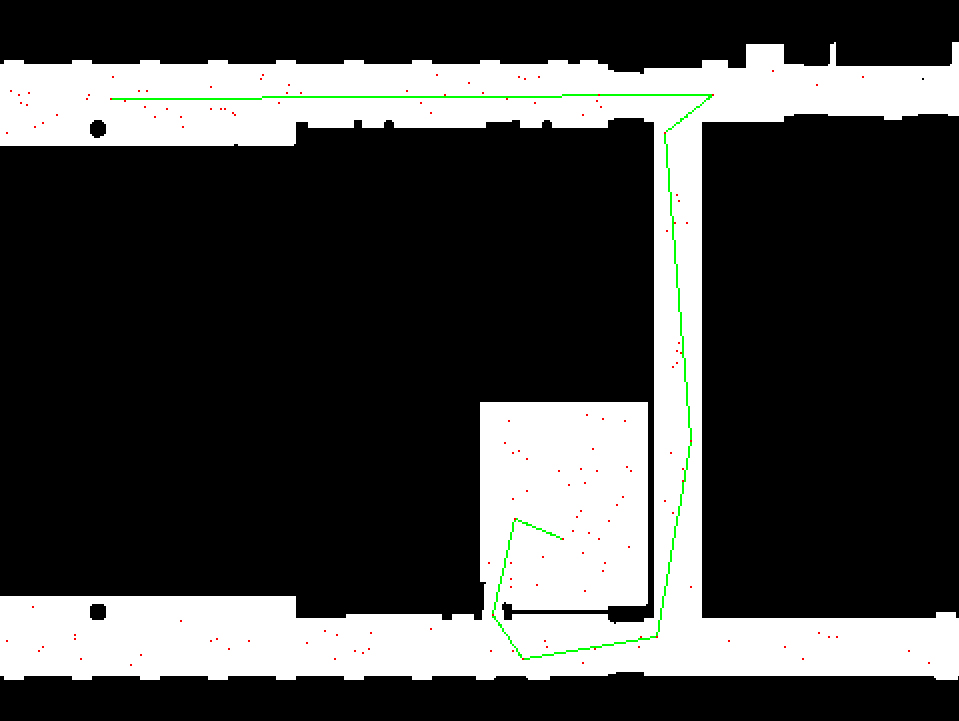
\includegraphics[scale=.4]{img/expath.jpg}
\caption{Example of a planned path in green starting from the upper hallway and ending in the robotics lab. The red dots are randomly chosen PRM points. The red dots along the green path are waypoints at which the robot will attempt to relocalize.}
\label{fig:expath}
\end{figure}


One downfall of the PRM is its random nature. For the purposes of this project we cannot manually pick and choose points in the obstacle map to use for path planning. Instead we must choose these points randomly. The only points that we ensure are chosen are points corresponding to the eight initial robot locations and the user-specified destinations. After the edges are determined we validate the PRM by ensuring that a path exists from each initial robot location to each destination point. Instead of checking each combination of initial robot location and destination point pairings, we just ensure that one long a path can be formed between all of these points. If this validation step fails, we generate new points and repeat the process by constructing a new PRM. If the number of random points to use is set too low, the validation step may fail multiple times, usually because it cannot create a valid path with enough buffer space to pass through the doorway into the robotics lab. Since we validate the map before the robot localizes or begins to move, it may wait in place for a half a minute or so depending on how long it takes to generate a valid PRM. Clearly, generating a valid PRM to in the initial stages of the program minimizes computation costs and planning time after the robot has been set in motion.

Another potential concern is the computational complexity of the path planning. We essentially use a brute force approach to try and determine all possible edges between all possible pairs of points. Thus, if there are $n$ points, the complexity is $O(n^2)$. If processing time is a concern, or computing resources are limited, then our program can be modified to only try and form connections between points that are within a certain distance of each other, or form connections between a point and its $k$ nearest neighbors. The problem with such a modification is that the paths generated may not ensure the fewest number of waypoints nor maximize the number of possible longest straight line paths.

If the robot is ever completely blocked in and cannot move forward for a period of time (which often happens when dealing with unforeseen obstacles and local minima in the potential field, see Section \ref{sec:robotmotion}), we update the obstacle map to account for the obstacle currently in front of the robot, update the PRM by adding the robot's current position as a new point and generating new edges, and replan the path starting at the robot's current position. Most often this results in the robot back-tracking to a point a few meters behind it and then attempting to move to a point slightly to the left or right of the obstacle so that it can navigate around it. Sometimes backtracking is not necessary and the robot just turns left or right, moves to a nearby waypoint, and then continues along its previously planned~path.

Note that this form of PRM path planning can be slightly inefficient. For example, in Figure \ref{fig:expath} it is unnecessary for the robot to traverse the full path between some pairs of waypoints (such as the pair of points at the top of the hallway to the right of the robotics lab and the pair of points within the robotics lab) in order to reach the final destination. Sometimes it may be more beneficial to have the robot abandon its current waypoint and plan a path to the next waypoint if it is closer and there are not obstacles in the way. This enhancement is a consideration for future work. 


\section{Potential Field Motion}
\label{sec:potential}

The robot navigates the path between each pair of waypoints by using potential field motion. This addresses the issue of obstacle avoidance because the robot will be repulsed by obstacles in its environment while being attracted to the goal. We chose potential field motion because we wanted to avoid using an evidence grid for path planning, thus the robot needs to be capable of avoiding obstacles in its environment without the constant need to explicitly replan the path each time an obstacle is encountered. In other words the robot needs to be more reactive so that it can handle minor unforeseen changes in its environment.

The major benefit of potential field motion is that in general the robot will appropriately navigate around obstacles and home-in on its current destination. Obstacles are sensed using the range finder and obstacles that are close to the robot have a stronger repulsive force than the obstacles further away from the robot, thus minimizing potential collisions. The further the robot is from its current destination, the stronger the attractive force. Thus, the robot is less likely to be thrown off target by obstacles that are further away from the destination than obstacles that are close to the destination. Also, the robot will slow down as it approaches the target, due to the decrease in attractive force, and theoretically stop at the desired position. 

Equations \ref{eq:fattx} - \ref{eq:fatty} are used to calculate the potential field attractive forces. Note that $cx$ and $cy$ are the current real-world x and y robot coordinates, respectively, $nx$ and $ny$ are the real-world destination x and y coordinates, respectively, and $katt$ is the attractive force constant.

\begin{equation}
fattx = -katt * (cx - nx)
\label{eq:fattx}
\end{equation} 
\begin{equation}
fatty = -katt * (cy - ny)
\label{eq:fatty}
\end{equation} 


Algorithm \ref{alg:frep} is used to calculate the repulsive forces.

\begin{algorithm}[H]
\caption{Calculation of Repulsive Forces}
\label{alg:frep}
\begin{algorithmic}[1]

\STATE{let $ranges$ be an array representing the current sonar ranges}
\STATE{let $p0s$ be an array representing the maximum distance away from the 
                      robot each range reading has an impact}
\STATE{let $kreps$ be an array representing the repulsive force constant of each sonar}
\STATE{let $ctheta$ be the robot's current orientation}
\STATE{$frepx = 0, frepy = 0$}
\FOR{each sonar $i$}
	\IF{$range[i] < p0s[i]$}
		\STATE{let $sonarangle$ be the relative angle of sonar $i$ to the robot}
		\STATE{$ frep = kreps[i] * (\frac{1}{range[i]} - \frac{1}{p0s[i]}) *(\frac{1}{range[i]^2}) $}
		\STATE{$ tmpfrepx = frep * cos(sonarangle)$}
		\STATE{$ tmpfrepy = frep * sin(sonarangle)$}
		\STATE{$ dirx = cos(ctheta + sonarangle)$}
		\STATE{$ diry = sin(ctheta + sonarangle)$}
		\STATE{$ tmpfrepx = sign(dirx) * tmpfrepx$}
		\STATE{$ tmpfrepy = sign(diry) * tmpfrepy$}
		\STATE{$ frepx = frepx + tmpfrepx $}
		\STATE{$ frepy = frepy + tmpfrepy $}
	\ENDIF
\ENDFOR

\end{algorithmic}
\end{algorithm}


Equations \ref{eq:fx} - \ref{eq:fy} are used to calculate the combined attractive and repulsive forces, which the robot converts to a directional vector to determine its current heading and speed.

\begin{equation}
fx = fattx + frepx
\label{eq:fx}
\end{equation} 
\begin{equation}
fy = fatty + frepy
\label{eq:fy}
\end{equation} 

Note that we needed to cap the attractive forces. This is because when the robot is far away from the destination the attractive forces can be very high and often overpower the repulsive forces of obstacles directly in front of the robot, causing it to attempt to plow through those obstacles.


\section{Hybrid Motion}
\label{sec:robotmotion}

Although in theory potential field motion sounds like a great idea, one encounters a few difficulties when trying to employ it. The first and foremost problem is falling victim to undesirable potential field minima. In the best case, the only minima in the environment is centered around the destination point, however, sometimes the repulsive and attractive forces acting on the robot will equal out and the robot will cease to move before reaching the destination. We have often observed cases where the robot will oscillate between a small set of poses and not make any progress. The literature states that it is possible to appropriately assign values to the attractive force constants, repulsive force constants, and other parameters ($katt, kreps, p0s,$ etc.) to prevent this from happening, but doing so is not possible if unforeseen obstacles are present in the environment (and it is also mathematically non-trivial). A reasonable approach would be to update these parameters when a new obstacle is detected, but we chose not to pursue that option. Another approach is to randomly alter the values of these parameters within some reasonable bounds in the hope that the local minima will dissipate, but we did not have much success doing so.

There were two specific situations in which potential field motion was the most problematic. The first situation is when the robot is attempting to navigate through a narrow passage with the destination in front acting as an attractive force and obstacles on the left and right acting as repulsive forces. Since the robot must pass very close to the obstacles their repulsive force is very strong and it overcomes the attractive force. The second situation is when the robot is moving along a straight line path and confronts a obstacle oriented perpendicular to that path. In this case the obstacle exerts a repulsive force directly opposing the attractive force. Thus, while the robot could easy move left or right to get around the obstacle, it has no forces directing it to do so, and it instead comes to a halt. Note that if these situations are encountered when the robot is run in simulation, the robot does not appear to stand still, rather it ``struggles" by quickly moving left and right at its maximum turning rate because of the large impact of the various opposing forces.

After many different attempts to get potential fields to overcome these issues, we decided that the best course of action would be to switch the robot over into wall-following mode if it encounters a situation in which it is not making any forward progress. Thus, we keep a counter for the number of iterations the robot does not move forward and once that exceeds a threshold we switch to wall-following mode for a predetermined number of iterations before switching back to using potential field motion. This approach is desirable since it gives objects (such as people or robots) time to move out of the way before we switch modes. This approach is very effective in simulation and even allows the robot to navigate through the door into the robotics lab as shown in Figure \ref{fig:expath}. We heuristically choose to the follow the wall (or obstacle) that exists between the robot and the destination, which may not always be the closest wall. Another way we attempt to reduce the occurrences of local minima is to rotate the robot in place to reach the desired heading before following the next path between waypoints.


\section{System Design}

All of the code for this project is written in Java. Java was chosen over C++ because of the ease-of-use when creating and updating the map GUI. The major disadvantage of a Java client implementation is that it does not receive periodic positional updates from the server as consistently as a C++ implementation would. This is most likely because of the overhead associated with Java being an interpreted language. As shown in Figure \ref{fig:uml}, there are five primary classes which compose the system.
 

\begin{figure}[H]
\centering
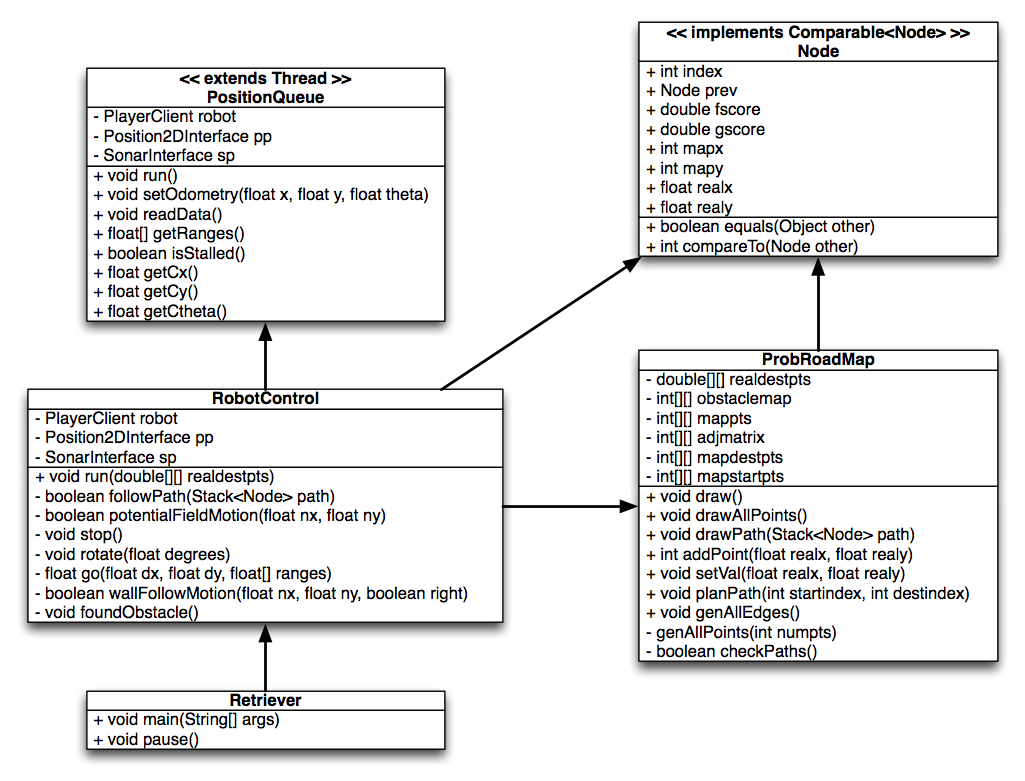
\includegraphics[scale=.6]{img/UML.jpg}
\caption{Overall system design.}
\label{fig:uml}
\end{figure}

\textbf{Primary Classes}
\begin{itemize}
\item{\textbf{Retriever} - main entry point into program, parses destination point file, creates RobotControl instance, and calls run() on it}
\item{\textbf{ProbRoadMap} - creates, maintains, and updates obstacle map, PRM points, and edges between those points; 
                       can plan a path using the A* algorithm}
\item{\textbf{RobotControl} - controls the movement of the robot; determines how to navigate the robot between two points; 
                      determines the next destination and uses a PRM to plan a path to it; updates the PRM when an obstacle is encountered 
                      that cannot be avoided}
\item{\textbf{PositionQueue} - thread that periodically reads positional information from the server to prevent buffer overflows and underflows}
\item{\textbf{Node} - simple object used to store information about a point in the environment; used by the A* algorithm for path planning}
\end{itemize}


\section{Experiments}

Localizing on the actual hardware was quite challenging, and at times a downright complete failure. We encountered two primary issues which inhibited successful localization on the hardware when compared to simulation. First, in real life it's very hard to place the robot at precise coordinates so that its initial sonar readings would match up nicely with those in simulation. While we attempted to address this issue by adding a little buffer in terms of comparing sonar readings to the expected values for each initial location, it still proved to be a headache, and did not work correctly in tests. The second issue is the infamous inaccuracy of the sonar readings. This proved to be a major headache and was the root of nearly all localization failures, and subsequently, relocalization failures at each waypoint. Since the sonar readings were somewhat sporadic and never quite the  same for the same robot position (even when the robot was completely stationary), it was very difficult to localize efficiently. Inaccurate odometer readings also led to relocalization problems. The robot would arrive at a waypoint and attempt to use its sonar readings to find the ranges of obstacles (i.e. walls) that it predicted would be in its immediate environment (according to the obstacle map). Inaccurate odometry led to issues linking real-world coordinates to map coordinates, and in turn which obstacles the robot expected to be in its immediate vicinity. Also, inaccurate sonar readings led to issues when the robot attempted to use nearby obstacles to gauge its offset from its desired position and update its odometry.

When dealing with the sonar, we observed that if the wall was close to perpendicular to the sonar emitting the sound, sonar readings were reasonably accurate; however, as the angles of incidence differed from the perpendicular, the readings became extremely erratic and quite unpredictable. Hence, it was very hard to deal with this issue reliably. Another serious issue we encountered during initial localization tests on the hardware was the presence of non-static obstacles. For example, if the robot needed to venture some distance before it could determine it's locale, and it was surrounded with people (such as curious freshmen), localization would fail. Modifying the localization code to account for this behavior would may have caused the robot to observe information about its environment for a very long time before finally deciding on its initial location, let alone visiting the desired destination points. While simple collision avoidance allowed the robot to prevent colliding with these obstacles, the robot was unable to determine whether the obstacles was static (and captured in its obstacles map) or otherwise. When localization and relocalization did work, the success of each was relative to what we considered success. Sometimes the robot would localize within half to a quarter of a meter its desired position.  These results were more hit or miss.

A great deal of time was spent attempting to get potential field motion working on the actual hardware. The first major issue was tweaking the attractive and repulsive force constants to come up with values for which the robot would behave reasonably. This proved to be difficult because of the second major issue: the sonar range finder readings were not consistent. Taking the same approach we did for the goTo assignment, and ignoring sonar readings believed to be inaccurate, caused the robot to move somewhat sporadically, causing it to quickly turn towards and away from approaching obstacles. We tried to mitigate this effect by taking multiple readings over 5 - 10 iterations for each sonar and basing our repulsive force calculations on the median value. In general that worked a little better, but the robot would not respond quickly enough to approaching obstacles. Reducing the maximum speed of the robot helped alleviate this problem.

One of the benefits of using potential field motion on the actual hardware was that we did not have to account for the acceleration or momentum of the robot too much as it navigated the environment. The robot would speed up if there were no obstacles ahead of it and slow down, and even stop, otherwise. Also, it was really nice that we did not have to take a predictive step to prevent the robot from overshooting its destination like we did for the goTo assignment. When the robot switched over into wall-following mode its behavior was much more stable. We used the same tried-and-true wall-following code that we used for the wall-following assignment and in general it worked reasonably well. It was also capable of navigating into the robotics lab door as long as it was traveling no faster than about 0.3 meters per second.

Table \ref{tab:simresults} summarizes the results of running three experiments in simulation and Table \ref{tab:realresults} summarizes the results of running the same three experiments on the actual hardware. TTL stands for ``time to localize". DTG stands for the final ``distance to goal" and represents how close the robot ended up near its intended destination. The starting positions correspond to the red, blue, and grey robots for experiments 1, 2, and 3, respectively. Total time does not consider the time it takes to build the PRM. \\

\begin{table}[h]
\footnotesize
\centering
\begin{tabular}{| c | c | c | c | c | c | c | c |}
\hline
{\#} & Start Pos. & End Pos. & Planned Dist.(m) & Actual Dist.(m) & TTL(s) & Total Time(s) & DTG(m) \\
\hline 
1 & (-15.5,12.0) & (7.5,1.0) & 33.43 & 33.14 & 1 & 83 & 0.26 \\
\hline 
2 & (7.5,-5.0) & (0.0,-7.0) & 21.38 & 20.91 & 34 & 122 & 0.49 \\
\hline 
3 & (-48.0,-10.5) & (-5.0,-10.5) & 43.05 & 43.05 & 1 & 96 & 0.40 \\
\hline
\end{tabular}
\caption{Simulation experiment results.}
\label{tab:simresults}
\end{table}

\begin{table}[h]
\footnotesize
\centering
\begin{tabular}{| c | c | c | c | c | c | c | c |}
\hline
{\#} & Start Pos. & End Pos. & Planned Dist.(m) & Actual Dist.(m) & TTL(s) & Total Time(s) & DTG(m) \\
\hline 
1 & (-15.5,12.0) & (7.5,1.0) & 34.06 & 40.54 & 5 & 130 & 0.31 \\
\hline 
2 & (7.5,-5.0) & (0.0,-7.0) & 21.40 & 23.07 & 45 & 318 & 0.45 \\
\hline 
3 & (-48.0,-10.5) & (-5.0,-10.5) & 43.02 & 50.18 & 5 & 123 & 0.21 \\
\hline

\end{tabular}
\caption{Real world experiment results.}
\label{tab:realresults}
\end{table}

Note that because there is a degree of randomness to the paths planned by the PRM approach, the results of running the experiments in simulation and the results of running the experiments on the hardware cannot be directly compared. Also, because each path consists of multiple waypoints, navigating a path to one destination is very similar to navigating a path to multiple destinations. All simulation experiments were run with the other 7 robots statically present with the exception of the robot that would normally occupy the destination point. Obstacles such as humans and chairs were encountered during each real world experiment, especially experiment 1 and 2. Note the large increase in total time from when experiment 2 was run in simulation to when it was in on the hardware. This is primarily due to the difficulty of the robot navigating through the robotics lab door frame. 


\section{Conclusion}

Overall we believe that potential field motion is a good choice for use with probabilistic road map path planning. This is because the paths provided by PRMs are not as precise as the paths provided by grid-based methods such as D*, therefore the robot must be capable of making more reactive decisions in response to environmental changes. For example, if the D* method is employed then the robot can quickly plan another path with a high degree of accuracy (depending on the granularity of each cell in the evidence grid). The D* method also produces cell-by-cell directional vectors. Alternatively, a PRM essentially provides an ordered listing of waypoints to visit with assurance that no known obstacles exist in between them. Once an obstacle is encountered in the PRM approach, a new point is added to the obstacle map, new edges are generated, etc. Clearly this path replanning process is more involved and time-consuming than the D* approach. Hence, the number of times necessary to replan the path should be minimized and the amount of variation that can be dealt with by the motion algorithm should be maximized.

Although the concept behind potential field motion is very simple, getting it to work properly is not because variables must be tuned properly to prevent local minima. In general we think that potential field motion is better suited for navigation through open environments with sparsely distributed obstacles. The third floor of the GCCIS building is more of a structured environment with medium to narrow-sized passageways and few known obstacles, except for pillars. 



\end{document}






